\section{Man against machine}
\label{sect:mam_study}
Here we set an experienced human scheduler up against a series of automated schedulers to see who wins.
description - likely problems assumptions errors how handled, input forms, what they did - notes from subject, how measured, results-comparison with other schedulers.

\subsection{Rational and introduction}
Selecting appropriate groups to perform is a complex task. There are many trade-offs to be made between the various competing preferences and constraints. When the schedule is heavily loaded, i.e. there are potentially more observations to perform than could be accomodated even under ideal conditions, the job of the scheduler becomes extremely difficult. A major problem is to determine just what those tradeoffs are - i.e. just how much more important is a high priority, non-urgent group relative to a medium priority urgent group?. It is because it is difficult to quantify these relative weights that we turn to the human scheduler. A human makes these sort of trade-offs on a daily basis - often with little knowledge they are doing it - if we set a human up to perform the task we might be able to deduce from what they have done and the choices they have made some of the rules they are using (often without realizing) and the relative weighting they employ. Additionally it was thought that it would be useful just to know if a human was in fact capable of \emph{beating} an automated scheduler in terms of the standard SQMs.


\subsection{Characterization of problem}
Plots of dmd and contention for the problem plus any relevant tabulated information.

\begin{figure}[htbp]
\begin{center}
    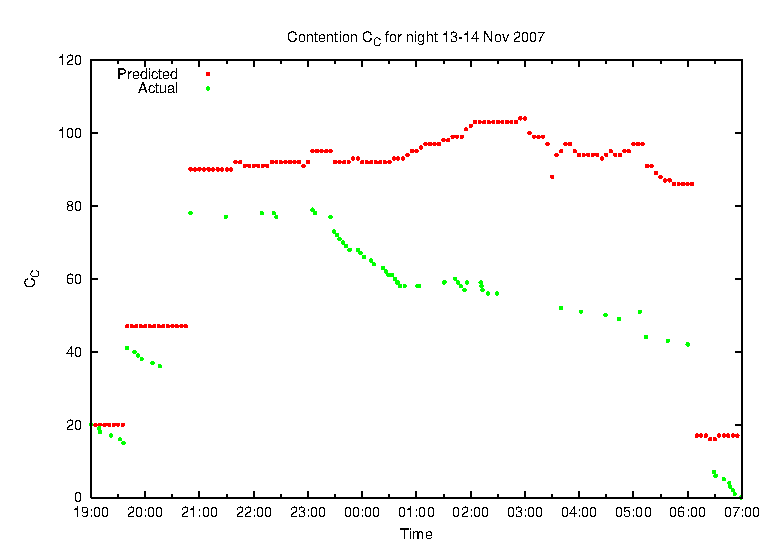
\includegraphics[scale=1.0, angle=0]{figures/mam/cont.eps}
\end{center}
\caption[Contention for night 13-14 November 2007.]
{Contention for night 13-14 November 2007 for H1 test. The two plots show the expected contention based on ODB content calaculated in advance and the actual contention derived during a typial scheduling run on the night.}
\label{fig:mam_h1_contention}
\end{figure}

\begin{figure}[htbp]
\begin{center}
    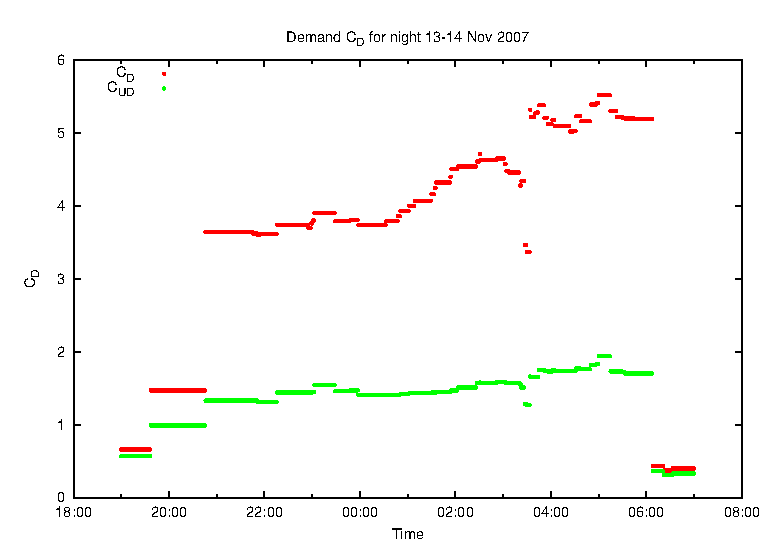
\includegraphics[scale=1.0, angle=0]{figures/mam/dmd.eps}
\end{center}
\caption[Demand for night 13-14 November 2007.]
{Demand for night 13-14 November 2007 for H1 test. The two plots show the overall and urgency-weighted demand.}
\label{fig:mam_h1_dmd}
\end{figure}

\subsection{Method of presentation}
What information is presented to the human scheduler.
Tables of crit and non-crit groups. What fields in table - explain what they are.
Explain how the human is restricted and how we relax some constraints e.g. elevation limit as HS cannot work this out easily for any given time.

\begin{description}
\item[Column  1] Group numeric ID - this is what the user enters into the seqence table.
\item[Column  2] Target RA.
\item[Column  3] Target dec.
\item[Column  4] Group name.
\item[Column  5] Timing (class and detail e.g. Monitor 12h, Interval 48h).
\item[Column  6] Moon constraint.
\item[Column  7] Seeing constraint.
\item[Column  8] Solar elevation constraint.
\item[Column  9] Priority (0-5, background, std).
\item[Column 10] Execution time (mins).
\item[Column 11] Urgency (No. of nights or critical).
\item[Column 12] Availability display, a simple pre-calculated plot of group observability during the night. 
\end{description}

\clearpage

\begin{landscape}

\begin{table}
\begin{center}
\caption{Example output from HumanSchedulerTestGenerator}
\begin{tabular}{|l|l|l|l|l|l|l|l|l|l|l|}
\hline
{\bf ID} & {\bf RA}    & {\bf Dec} & {\bf Name} & {\bf Timing} & {\bf Moon}  & {\bf Seeing} & {\bf Night}   & {\bf Priority}    & {\bf Exec}   & {\bf Urgency} \\
\hline
G\_448  &22:41:55.90  &20:15:42.00  &UCM\_galaxies\_6&FLEXBL  &DARK &AVER  &       &1 &39.63M  &11 \\
\hline
G\_449  &23:51:25.70  &24:24:12.00  &UCM\_galaxies\_18&FLEXBL &DARK &AVER  &       &1 &39.63M  &12 \\
\hline
G\_450  &23:22:20.90  &23:0:42.00&UCM\_galaxies\_14  &FLEXBL  &DARK &AVER  &       &1 &39.63M  &12 \\
\hline
G\_452  &22:58:50.00  &20:17:54.00  &UCM\_galaxies\_7&FLEXBL  &DARK &AVER  &       &1 &39.63M  &11 \\
\hline
G\_453  &23:31:48.50  &24:44:6.00&UCM\_galaxies\_17  &FLEXBL  &DARK &AVER  &       &1 &39.63M  &12 \\
\hline
G\_455  &23:5:25.50&21:9:42.00&UCM\_galaxies\_4&FLEXBL        &DARK &AVER  &       &1 &39.63M  &12  \\
\hline
G\_466  &22:53:57.74  &16:8:53.56&2251  &MONITR 168H [167]    &DARK &AVER  &       &1 &7.8M   &2  \\
\hline
G\_469  &22:2:43.291  &42:16:39.98  &2200 &MONITR 168H [167]  &     &AVER  &       &1 &7.8M   &2 \\
\hline
G\_470  &2:38:38.93&16:36:59.28  &0235 &MONITR 168H [167]     &DARK &AVER  &       &1 &7.8M   &2  \\
\hline
G\_471  &12:29:6.70&2:3:8.60  &1226 &MONITR 168H [167]        &     &AVER  &       &1 &7.8M   &2  \\
\hline
G\_472  &8:54:48.90&20:6:30.64&0851 &MONITR 168H [167]        &DARK &AVER  &       &1 &7.8M   &2  \\
\hline
G\_476  &0:42:49.64&41:15:26.50  &ANGM31  &MONITR 2.5H [2]    &     &POOR  &       &2 &33.4M   &CRIT  \\
\hline
G\_481  &14:17:59.60  &25:6:53.00&5548\_opt&MONITR 168H [120] &     &POOR  &ASTR   &2 &3.13M  &3  \\
\hline
\end{tabular}
\end{center}
\end{table}

\end{landscape}

\subsection{HS results}
Table of HS results for various metrics.

\subsection{Method of simulation}
Explain how we perform the simulations - cut-down architecture to mimic the information available to the HS. ie the automatic scheduler knows what the human knows.

\subsection{BDS simulation results}
Plot of comparison of various metrics against scoring function.

\begin{figure}[htbp]
\begin{center}
    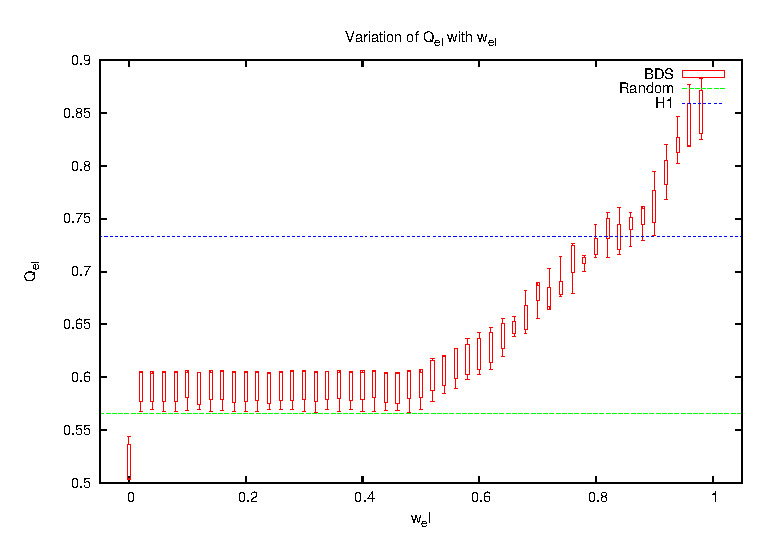
\includegraphics[scale=1.0, angle=0]{figures/mam/cmp_el.eps}
    \caption[Variation of $Q_{el}$ with $w_{el}$.]
      {Variation of quality metric $Q_{el}$ with $w_{el}$ for BDS schedules scored using combination of $w_{el}$ and $w_{pr}$.}
\label{fig:mam_cmp_el}
\end{center}
\end{figure}


\begin{figure}[htbp]
\begin{center}
    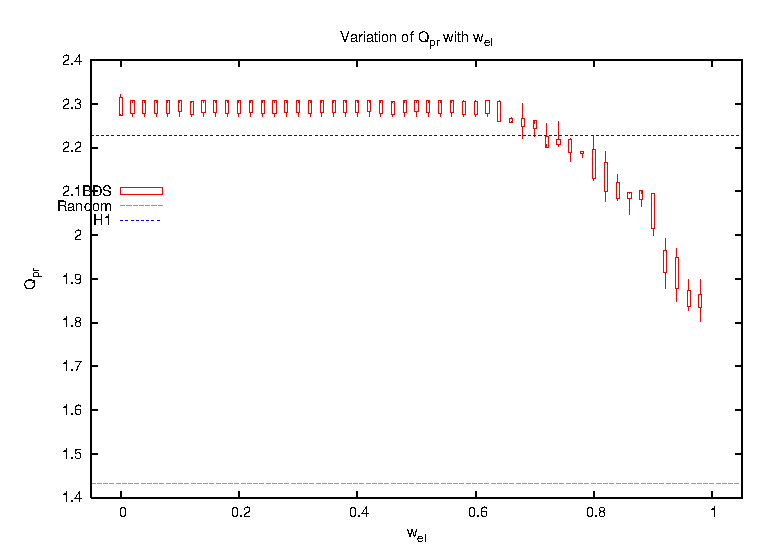
\includegraphics[scale=1.0, angle=0]{figures/mam/cmp_pr.eps}
    \caption[Variation of $Q_{pr}$ with $w_{el}$.]
      {Variation of quality metric $Q_{pr}$ with $w_{el}$ for BDS schedules scored using combination of $w_{el}$ and $w_{pr}$.}
\label{fig:mam_cmp_pr}
\end{center}
\end{figure}



\begin{figure}[htbp]
\begin{center}
    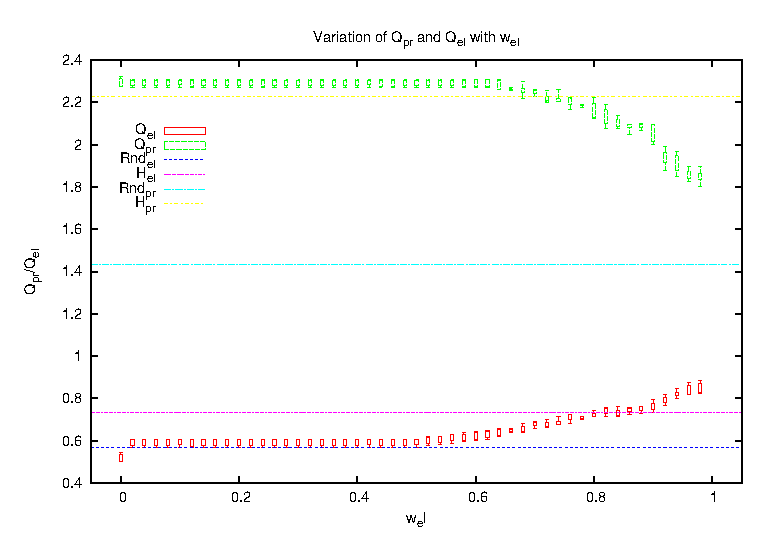
\includegraphics[scale=1.0, angle=0]{figures/mam/cmp_elpr.eps}
    \caption[Variation of $Q_{el}$ and $Q_{pr}$ with $w_{el}$.]
      {Variation of quality metrics $Q_{el}$ and $Q_{pr}$ with $w_{el}$ for BDS schedules scored using combination of $w_{el}$ and $w_{pr}$.}
\label{fig:mam_cmp_elpr}
\end{center}
\end{figure}

\begin{figure}[htbp]
\begin{center}
    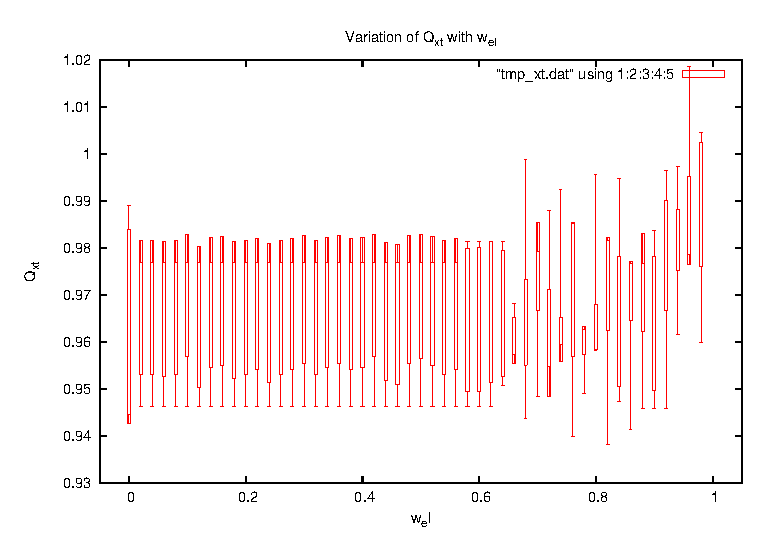
\includegraphics[scale=1.0, angle=0]{figures/mam/cmp_xt.eps}
    \caption[Variation of $Q_{xt}$ with $w_{el}$.]
      {Variation of quality metric $Q_{xt}$ with $w_{el}$ for BDS schedules scored using combination of $w_{el}$ and $w_{pr}$.}
\label{fig:mam_cmp_xt}
\end{center}
\end{figure}


And now a table showing the results.

\begin{table}
\begin{center}
\caption{Results of BDS simulations and Human scheduler}
\begin{tabular}{|l|rrrrrrrrr|}
\hline
{\bf metric} & {\bf $h_1$} & {\bf $B_{el}$} &  {\bf $B_{pr}$} & {\bf $B_{rn}$} & {\bf $B_{td}$} & {\bf $B_{2,8}$} & {\bf $B_{5,5}$} & {\bf $B_{8,2}$} & {\bf $B_{rnd}$}\\
\hline
{\bf $Q_{el}$} & 0.77 & 0.88 & 0.52 & 0.36 & 0.4  & 0.59 & 0.59 & 0.72 & 0.56 \\
{\bf $Q_{pr}$} & 2.34 & 1.87 & 2.29 & 1.73 & 1.54 & 2.3  & 2.3  & 2.16 & 1.43 \\
{\bf $Q_{sm}$} & 0.28 & 0.3  & 0.26 & 0.28 & 0.32 & 0.25 & 0.25 & 0.25 & 0.33 \\
{\bf $Q_{lm}$} & 0.71 & 0.8  & 0.68 & 0.82 & 0.92 & 0.64 & 0.64 & 0.7  & 0.86 \\
{\bf $Q_{rn}$} & 0.67 & 0.48 & 0.4  & 0.58 & 0.4  & 0.47 & 0.47 & 0.45 & 0.35 \\
{\bf $Q_{td}$} & 0.07 & 0.06 & 0.05 & 0.1  & 0.12 & 0.06 & 0.06 & 0.05 & 0.08 \\
{\bf $Q_{xt}$} & 0.99 & 0.99 & 0.96 & 0.99 & 1.0  & 0.96 & 0.97 & 0.96 & 1.0  \\
\hline
\end{tabular}
\end{center}
\end{table}


\subsection{LAS simulation results}
extra features - bg selection thresh - other wise stay idle, overun thresh frac of group in horizon


\subsection{Analysis and comparison}

\subsection{Conclusions}
